\chapter{Synthesizing Data for Object Detection on \acp{MAV}}
\label{sec:training}

Machine learning relies on the assumption that a general concept can be extracted from a limited set of examples. In Supervised Machine Learning, the set of examples $X$ is augmented with a set of labels $Y$ that describes task dependent information that is present in the sample. For Object Detection this could be the coordinates of the bounding box that surrounds the object of interest. The goal is to learn a hypothesis $h$ from a source set $D_S = \{X_{S},Y_{S}\}$ such that it can be applied on a target set of unknown examples $D_T = \{X_{T}\}$ to obtain the corresponding target labels:

$$
h(X_T)\rightarrow Y_T
$$ 

Whether $h$ is performing well, can be evaluated by splitting $D_S$ in a training and test set. $h$ is learned using the full information of the training set and applied on the test set. By evaluating a performance metric $m$ on the models output, the expected performance of $h$ on $D_T$ can be estimated and allows to evaluate whether model and dataset are suitable for the task.
			
In this setting it is assumed that the samples in $S$ and $T$ are \ac{i.i.d.}. However, when $S$ is synthesized, this assumption is violated as $S$ will share properties with the real data but only to the extent that they can be modelled during creation. For example a graphic engine can not fully capture visual properties of all materials and light sources. Furthermore, the environmental conditions for applications of the method such as at the \ac{IROS} 2018 Autonomous Drone Race are unknown and can be significantly different to the ones used at training time. Such a setting, in which $S$ only shares a subset of properties with $T$, is also referred to as a domain shift scenario. The goal is to create source domain $S$ and find a concept $h$ that maximizes its performance $m_T$ in the target domain. It can be summarized in:

$$
\text{arg}\max\limits_{h,S} m_T
$$

In order to evaluate whether the generated data is suitable domain shifts on different levels are mode

The conducted research focuses on \ac{CNN}-based object detection as they are investigated in this thesis. This chapter investigates data generation while the exact model is described in \Cref{sec:object_detection}.

The relevant question to be investigated in this chapter is the following:

\textbf{How can data be generated to train a detection model for \ac{EWFO} detection on a \acp{MAV}?}

\begin{enumerate}
	\item[\textbf{RQ1.1}]What are the implications of the properties of \acp{EWFO} when synthesizing data?
	\item[\textbf{RQ1.2}]What are the properties of the target domain, namely the \ac{FPV} camera of a \ac{MAV} in a GPS denied scenario?
	\item[\textbf{RQ1.3}]Can target domain knowledge be used to improve model performance/simplify model complexity ?
	\item[\textbf{RQ1.4}]How can data be generated in a way that the trained model is robust against expected domain shifts?
\end{enumerate}

RQ1.1 Will be answered by comparing the implications of domain properties on \ac{EWFO} and a standard object. RQ1.2 will be answered by analysing example datasets of a target domain. For RQ1.3 and RQ1.4 several domain properties are defined. The questions will be answered by choosing a state of the art method for object detection and training it with varying properties in $D_S$. By evaluating $m_S$ on synthetic data and $m_T$ on real images the influence of these properties will be measured.

The remaining parts of this chapter are structured as follows: \Cref{sec:training:related} discusses relevant related work. \Cref{sec:training:meth} describes the used methodology. Based on the gained insights \Cref{sec:training:hypothesis} formulates several hypotheses to be investigated. \Cref{sec:training:experiments} outlines the experiments conducted to evaluate the formulated hypotheses. \Cref{sec:training:results} describes the obtained results. \Cref{sec:training:conclusion} discusses the results and answers the research question.

\section{Related Work}
\label{sec:training:related}

Using synthetic images to train Machine Learning models has a long tradition in Computer Vision especially for tasks where not many example images are available or the ground truth labelling is expensive. Methods vary from changing low level properties of images like brightness or scale over pasting 3D-models of objects on real backgrounds to rendering full 3D-environments. Other publications show how the incorporation of sensor effects is important when generating data. However, most of these methods can be combined in different pipelines. Therefore most publications do not use on particular approach but different combinations. The related approaches are categorized in on which image level they operate.

\subsection{Augmenting Real Data}

\subsubsection{Low-Level Image Augmentation}

Low-Level Image Augmentation applies transformations on the samples of a given dataset. It is a common part of current Computer Vision pipelines.

\citeauthor{Krizhevsky2012a} \cite{Krizhevsky2012a} use PCA to incorporate colour variations. \cite{Howard2013} shows how several image transformations can improve the performance of a Classification model. In Object Detection \cite{Redmon} use random scaling and translation of the input image, as well as random variations in saturation and exposure. \citeauthor{Liu} \cite{Liu} additionally crop and flip the image with a certain probability. The common aim of these methods is to make the model more invariant towards changes in the augmented properties.

In contrast \citeauthor{Carlson2018}\cite{Carlson2018} augment the image based on a physical camera model. The proposed pipeline incorporates sensor and lens effects like chromatic aberration, blur, exposure and noise.

Low-Level Image Augmentation is a comparatively cheap method to generate a lot of data. However, it cannot create totally new samples or view points. Furthermore, it cannot change the scene in which an object is placed. Therefore it is restricted to some extent to the dataset that to be augmented.

In this work only the dataset of one room is available which is too small to train a model for multiple rooms with different environmental conditions. Hence, low-level image augmentation cannot be the only method for data generation.

\subsubsection{Augmenting Real Images with 3D - Models}

If a 3D-model of an object is available, it can be placed on real images to artificially create or increase a dataset. 

Several publications demonstrate the usefulness of this method in Object Detection \cite{Girshick2013}, \cite{Peng}.

While the previous methods simply place the object in a scene \citeauthor{Rozantsev} \cite{Rozantsev} propose to estimate rendering parameters first.

A comparable work has been done in \cite{Madaan2017} to detect wires based on synthetic data. However, the experiments focus on a single domain, namely wires in the sky and thus the variations in background are comparatively small.

In contrast augmenting the images on a low-level this method allows to generate new view points and does not require original images to augment. However, the created image is likely to be relatively artificial as for example light conditions and shadows are not align with the background scene. Furthermore can the object be placed in quite arbitrary positions and thus violate geometric and physical properties that are present in real images. 


\subsection{Fully Synthesizing Data}

\cite{Sadeghi2016,Hinterstoisser2017,Krizhevsky2012a}

While training models only in a simulated environment is common for Control tasks, it is less popular in Computer Vision as often the quality of graphic engines is too poor or the rendering is very time consuming. However, the advances in Computer Graphics and faster processing technologies nowadays allow the generation of more realistic images and various studies tried to incorporate these samples in their training process.

\cite{Ros2016, Gaidon2016} are fully rendered datasets used for Computer Vision. 

\cite{Johnson-Roberson2016} training in simulation only.

\cite{Tobin2017} was one of the first publications that used only synthetic images for the task of Object Localization. The proposed method \ac{DR} uses a high degree of randomization when rendering the image. Thus a model has to learn a general representation, that can also be applicable in the real world. \cite{Tremblay2018a} extends the approach to object detection.

The data is generated by a graphical engine. The following properties of the scene and the object are varied \cite{Tremblay2018a}:

\begin{enumerate}
	\item number, type and texture of objects of interest
	\item number, types, colours, scales of irrelevant objects (distractors)
	\item background image
	\item camera pose
	\item light sources
	\item visibility of ground plane
\end{enumerate}

An advantage of \ac{DR} is its ease of implementation and use, no assumptions about the target distribution have to be made neither are samples or labels of the target domain required. However, the method can fail to capture important patterns if the randomization is too strong. For example the movement pattern of a \ac{MAV} is ignored when placing the camera randomly.


\subsection{Augmenting Synthetic Data}

\subsection{Others}
Approaches that require samples of the target domain \cite{Chen2018c} \cite{Xu2017} \cite{Inoue} 

\cite{Peng2017} includes task-irrelevant samples and a source classifier to make the final network robust (?). Called zero-shot domain adaptation as no samples of the target domain are required.


\section{Methodology}
\label{sec:training:meth}

In the following methods used in this thesis are described. We define several domain properties and model them during data generation.

The models are implemented in a toolchain that applies the different steps. An overview can be seen in \Cref{fig:training:toolchain_datagen} \todo{Put example images}. The individual steps are described in the following.

\begin{figure}[htbp]
	\centering
	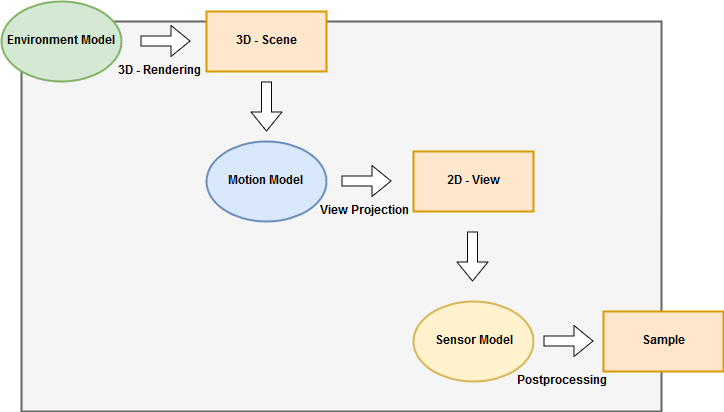
\includegraphics[width=\textwidth]{fig/Toolchain_datagen}
	\caption{Overview of the data generation process. The environment model determines background and lightning conditions and produces a 3D-Scene. The motion model determines the camera pose and location and thus the view point. Projecting the 3D-Scene on the image plane of the camera delivers the 2D-View. A final post processing step incorporates sensor and lens effects.}
	\label{fig:training:toolchain_datagen}
\end{figure}

\subsection{Scene Generation}
\label{sec:training:scene}
We define environment properties as illumination and background. For example a scene can be set outdoor in the forest at night or indoor with artificial light sources. Two methods are used two create an environment.

\subsubsection{Pasting a 3D-Model on Real Images}

Similarly to several methods in literature \cite{Girshick2013, Peng, Rozantsev} a 3D-Model of the \ac{TO} is pasted on real images.

The 3D-Model is provided by TODO and a tool to render these models is implemented using OpenGL. A scene with black background is created and several objects are placed on a virtual ground plane with different rotations to each other. Additionally light sources are placed at different locations and with different intensities. The exact light model is part of OpenGL and will not be further discussed in this thesis. 

After creating a scene the black background is replaced with an image obtained from a dataset. As the light conditions between background image and \ac{TO} are different, the created image can be quite artificial. Hence a postprocessing step applies a Gaussian blur kernel along the edges of the \ac{TO}. This leads to a better embedding of the \ac{TO} in the background.
Examples can be seen in \Cref{fig:random_bg}

The parameters and locations of objects and light sources as well as the selected backgrounds are parameters of the implemented tool that can be varied when creating a dataset.

\begin{figure}[hbtp]
	\centering
	\begin{minipage}{0.49\textwidth}
		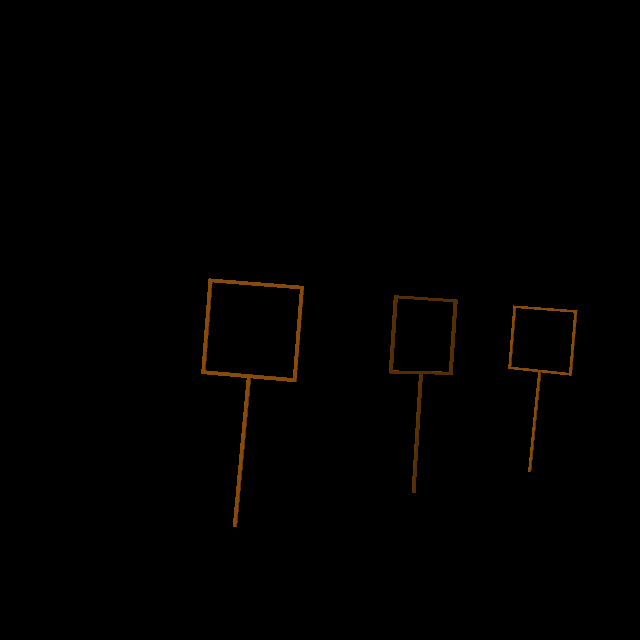
\includegraphics[width=\textwidth]{fig/shot}
	\end{minipage}
	\begin{minipage}{0.49\textwidth}
		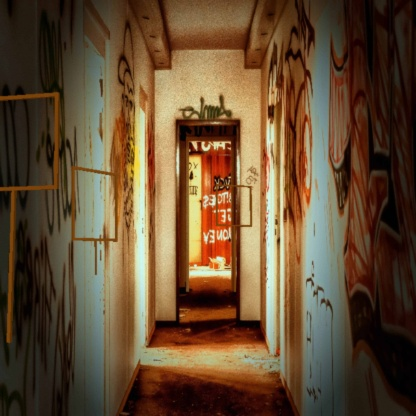
\includegraphics[width=\textwidth]{fig/random_bg2}
	\end{minipage}
	\caption{Examples for pasting the 3D-Model on various backgrounds. A scene with background is rendered (left), subsequently the black background is replaced with an image from a dataset.}
	\label{fig:random_bg}
\end{figure}

\subsubsection{Full Rendering of a Scene}

Following \cite{Ros2016, Gaidon2016, Johnson-Roberson2016, Tobin2017, Tremblay2018a} the second approach to create a scene is fully rendering the environment using a graphic engine, namely the UnrealEngine including the AirSim plugin.

The UnrealEditor allows to manually create environments and provides high quality rendering of objects, textures and light conditions. In total three environments, namely three indoor scenarios are created. This resembles GPS-denied scenarios as they are targeted in this thesis. Within the environment the light conditions, background textures, object locations can be changed manually.

In total three base environments are created. Examples can be seen in \Cref{fig:environments}.

\begin{figure}[hbtp]
	\centering
	\begin{minipage}{0.49\textwidth}
		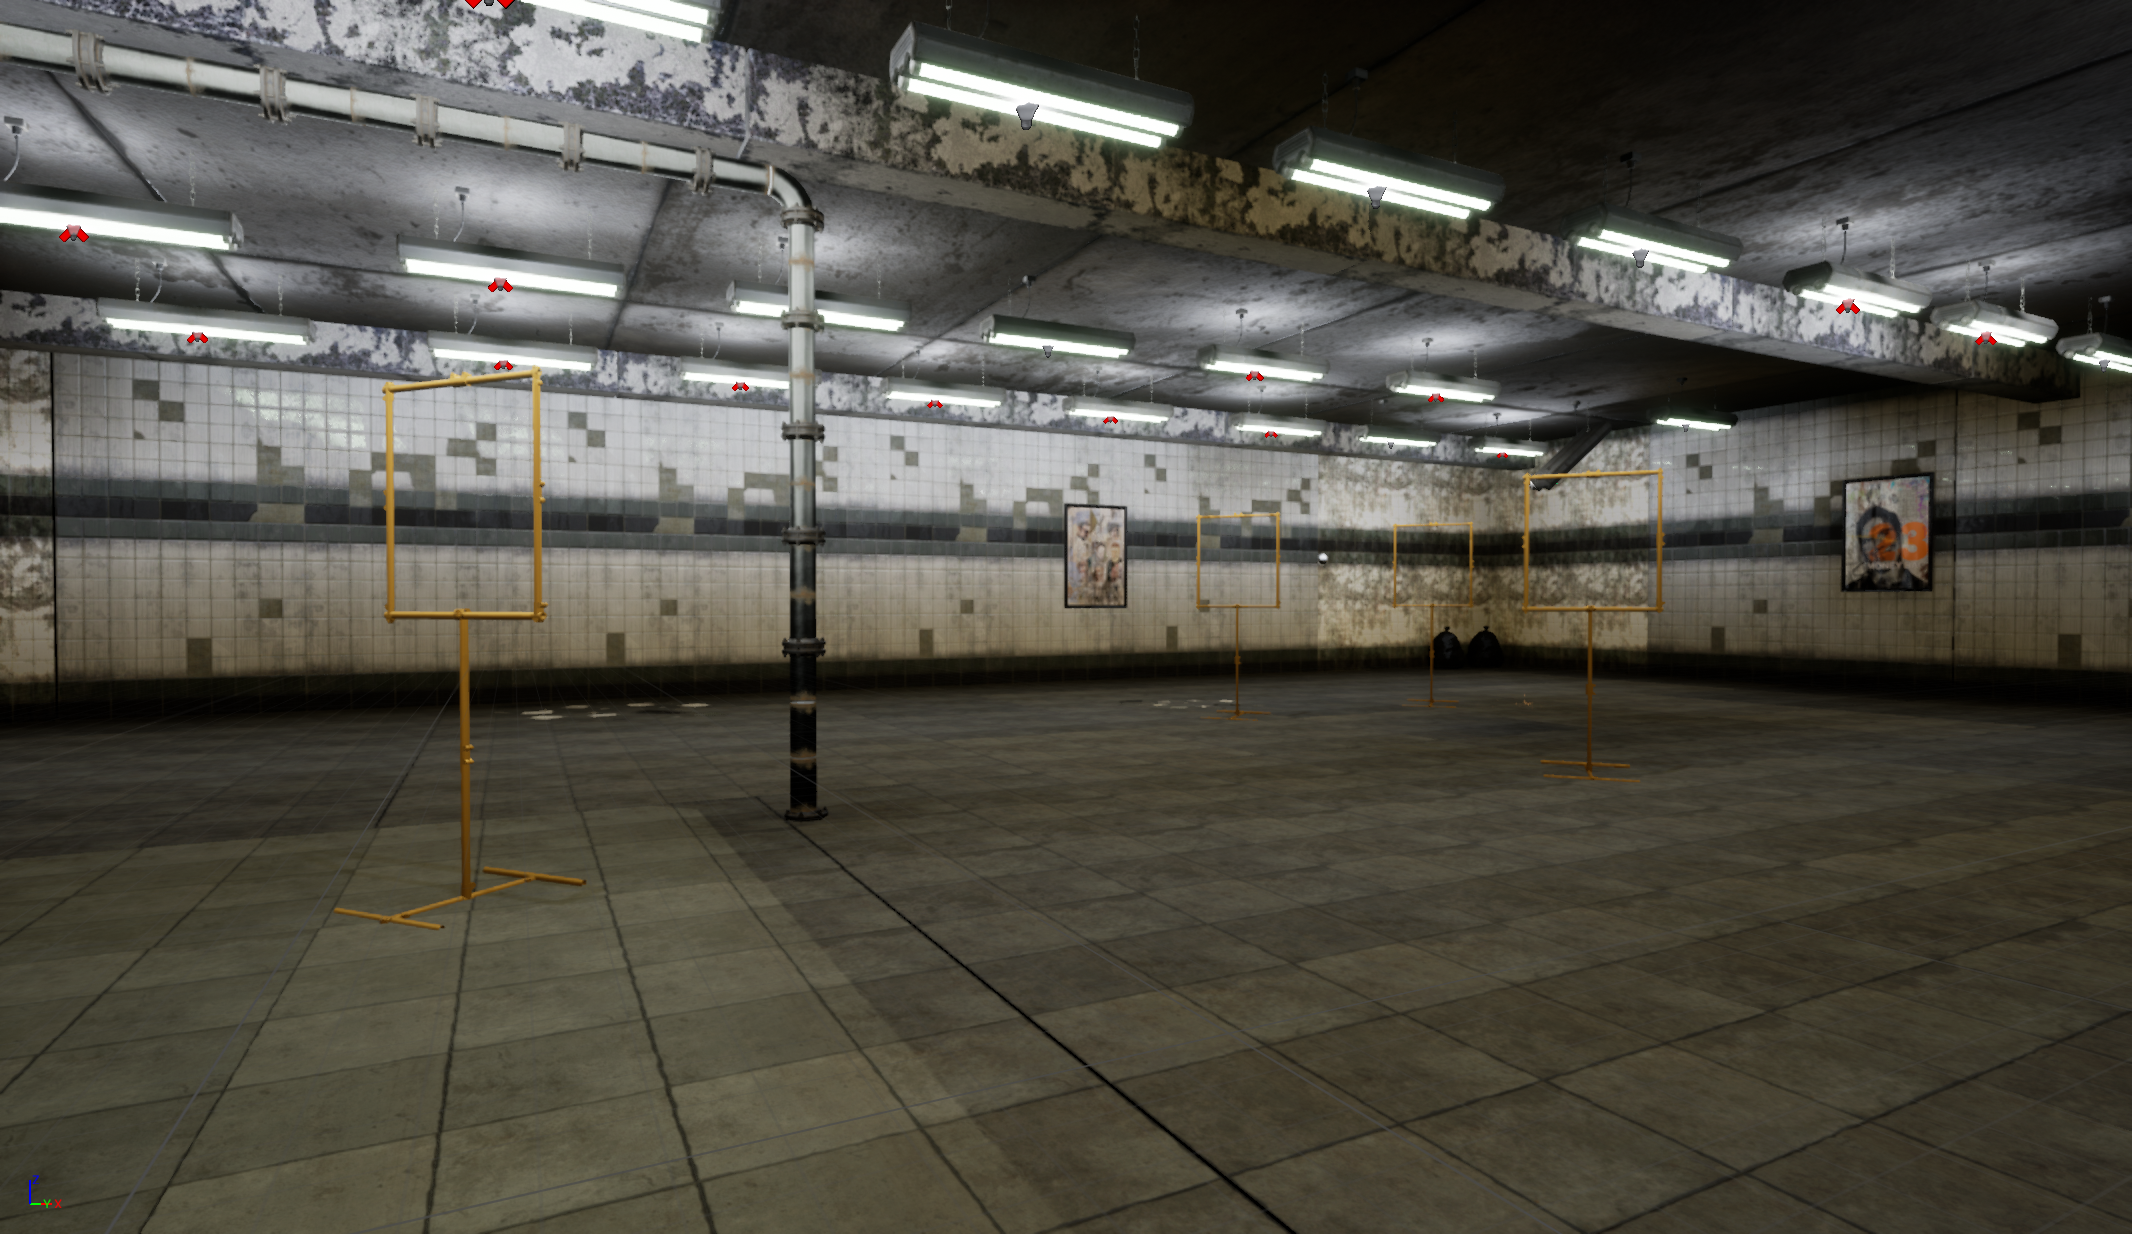
\includegraphics[width=\textwidth]{fig/basement_perspective}
	\end{minipage}
	\begin{minipage}{0.49\textwidth}
	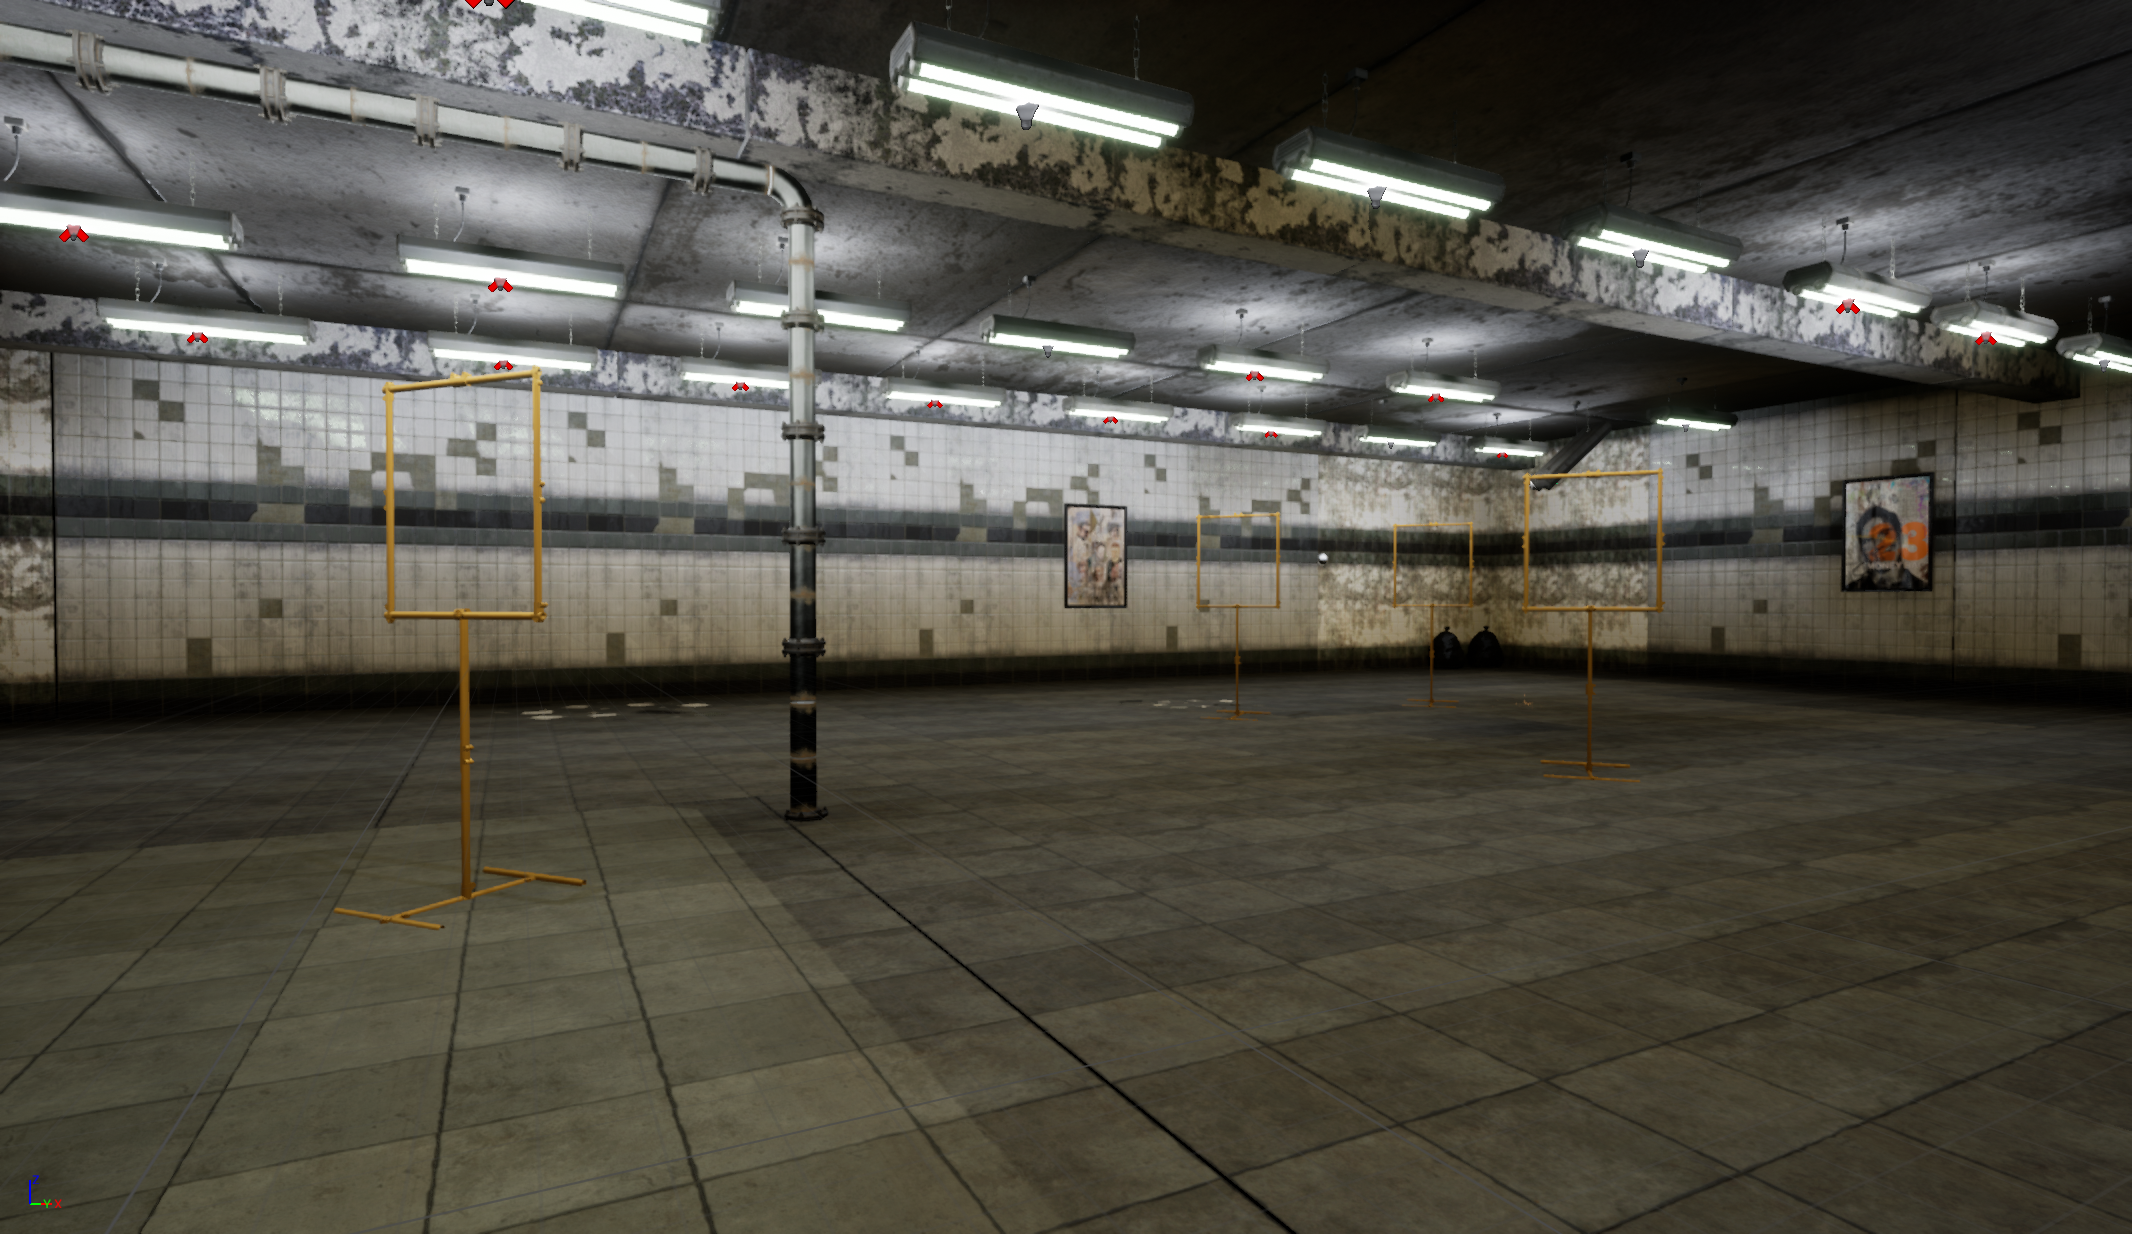
\includegraphics[width=\textwidth]{fig/basement_perspective}
\end{minipage}

\begin{minipage}{0.49\textwidth}
	\includegraphics[width=\textwidth]{fig/daylight_perspective}
\end{minipage}
\begin{minipage}{0.49\textwidth}
	\includegraphics[width=\textwidth]{fig/daylight_perspective}
\end{minipage}

\begin{minipage}{0.49\textwidth}
	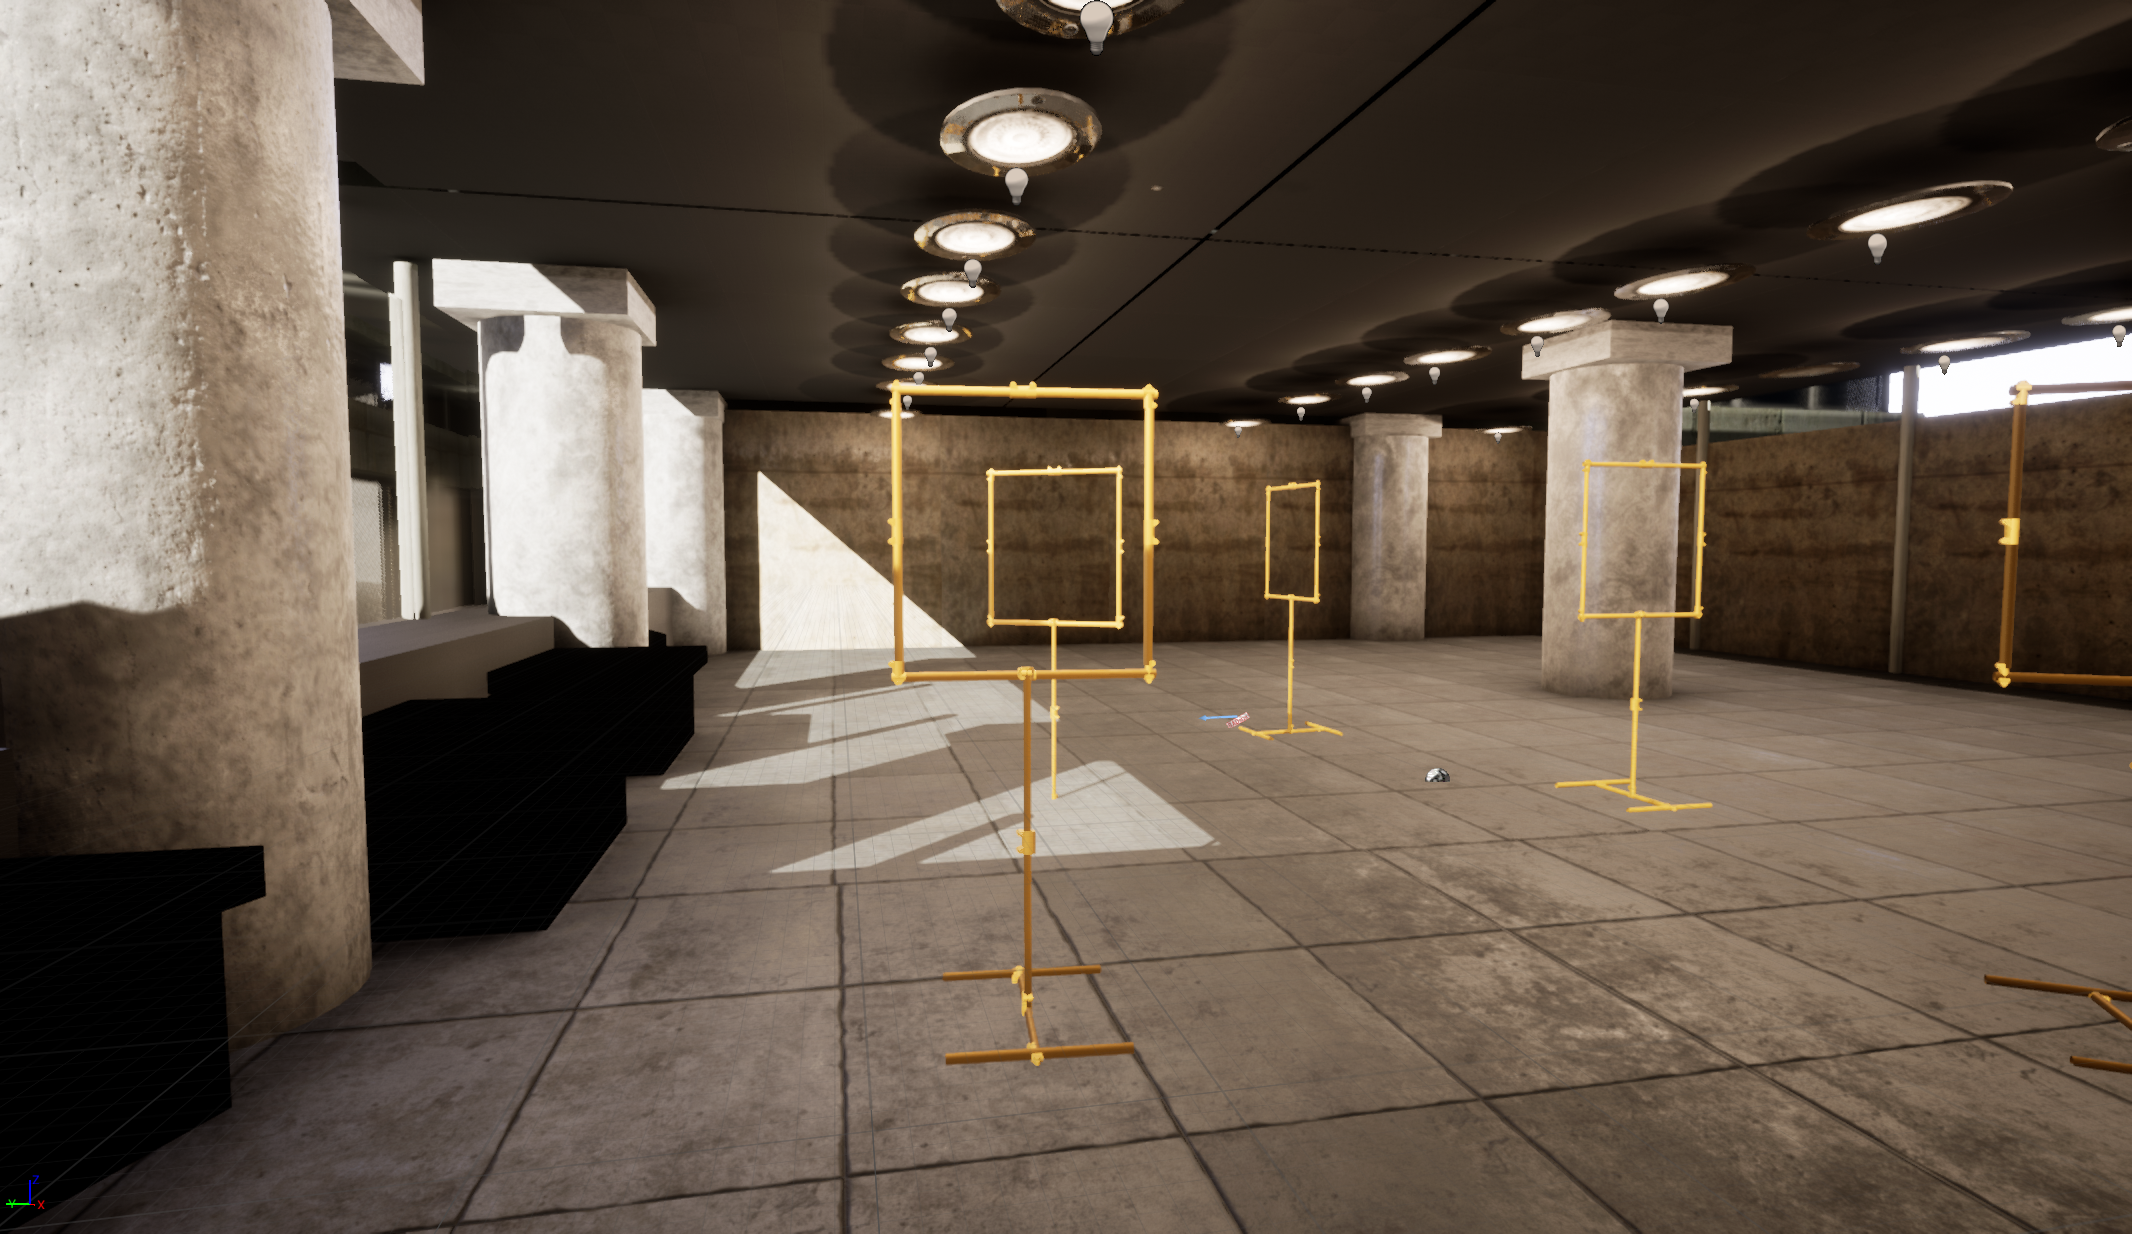
\includegraphics[width=\textwidth]{fig/iros_perspective}
\end{minipage}
\begin{minipage}{0.49\textwidth}
	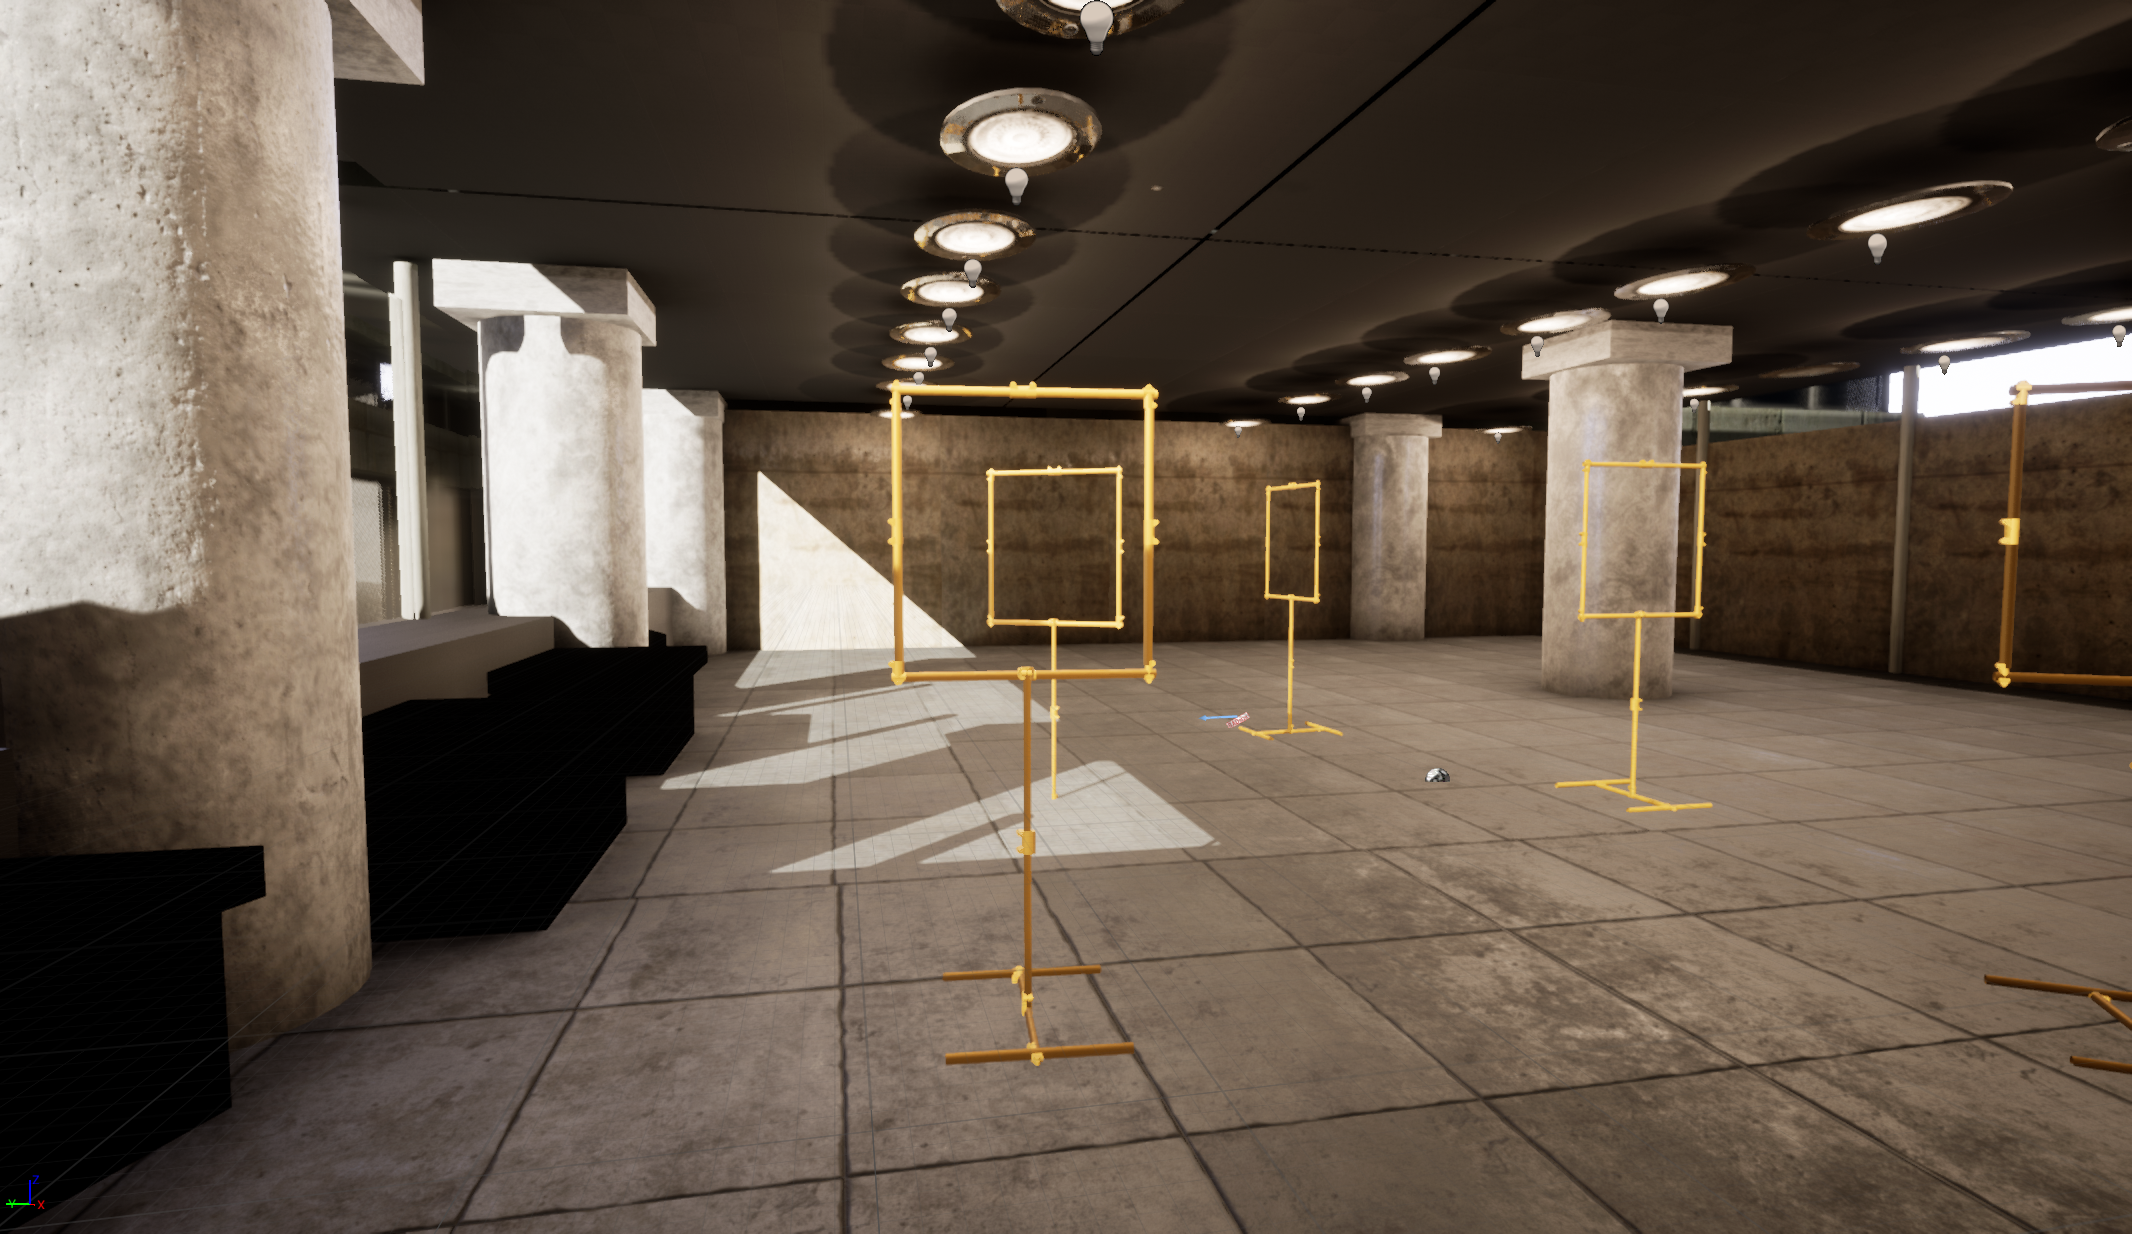
\includegraphics[width=\textwidth]{fig/iros_perspective}
\end{minipage}
\caption{Base environments when rendering a full scene. From top to bottom: \textit{Basement}, \textit{Daylight}, \textit{IROS}.}
\label{fig:environments}
\end{figure}

\subsection{Camera Placement}

The motion model refers to the camera's point of view. For the implemented tools in \Cref{sec:training:scene} the camera view point can be set during data creation. The camera pose is determined by:

$$
\text{Translation: }t = [x y z] \text{ and Rotation: } r = [\phi, \theta, \psi]
$$
Where the left-handed coordinate system is used with $z$ pointing in the image.

\subsubsection{Random Placement}
	
The value for each dimension of $r$ and $t$ are drawn from a probability distribution. The chosen distributions have to follow certain limitations, for example the gate should still be visible in most images.
	
\subsubsection{Quad-rotor Model}
	
$r$ and $t$ follow a the motion model of a quad-rotor \ac{MAV}.  The development of this model has not been done within this thesis but is summarized here for completeness: \todo{put shuos model here}.

Using this motion model, the camera follows a certain trajectory through the 3D-Environment. Storing the current image at a frequency of 2 Hz creates the corresponding samples.
	
\subsection{Post-processing}

\subsubsection{Model-based augmentation}
In the real world camera and lens have significant influence on the image appearance as well as the performance of neural networks \cite{Andreopoulos2012,Dodge2016a}. In order to model these effects a post-processing step is applied on the images obtained in the previous steps. The experiments in \cite{Carlson2018} show how such a step can be particularly beneficial when applied on artificially generated data. 

Inspired by \cite{Carlson2018} the model for chromatic aberration, exposure, blur and noise is included. However, on the camera of the \ac{MAV} we assume that we can process the raw image signal. Hence, no model for information loss due to post-processing is applied. Instead all images are converted into YUV-colour space, a format that is obtained from most visual sensors. The pipeline is extended by two models: (1) A model for lens distortion since \ac{MAV} often used wide angle lenses to increase their \ac{FoV}; (2) A model for motion blur since fast camera movements are to be expected.

The post-processing pipeline is summarized as:

\begin{equation}
	I' = \phi_{noise}(\phi_{exposure}(\phi_{FocusBlur}(\phi_{MotionBlur}(\phi_{Chrom.}(\phi_{Lense}(I))))))
	\label{eq:postprocess}
\end{equation}

The individual models are described in the following.

\paragraph{Lens Distortion}

\todo{Explain what lense does and its effects}

Lens distortion is applied using the model for wide-angle lenses from \cite{Vass}. It models the \textit{removal} of lens distortion as combination of radial and non-radial part, that is approximated with a second order Taylor expansion:

\begin{equation}
\begin{pmatrix}
	p_x' \\
	p_y'
\end{pmatrix} = \begin{pmatrix}
p_x(1 + \kappa_1 p_x^2 + \kappa_1 (1 + \lambda _x)p_y^2 + \kappa_2(p_x^2 + p_y^2)^2) \\
p_y(1 + \frac{\kappa_1 }{s}p_x^2 + \frac{\kappa_1}{s} (1 + \lambda _y)p_y^2 + \frac{\kappa_2}{s}(p_x^2 + p_y^2)^2)
\end{pmatrix} 
\label{eq:distortion}
\end{equation}
Where:
\begin{itemize}
	\item $p_x'$ and $p_y'$ are the undistorted coordinates.
	\item $\kappa_1$ controls the primary distortion (default 0)
	\item $\kappa_2$ controls the secondary distortion (default 0)
	\item $s$ controls the squeeze factor (default 1)
	\item $\lambda_x$ and $\lambda_y$ controls asymmetric distortion (default 0)
\end{itemize}
 
Applying the lens distortion to an image is done using the inverse of \Cref{eq:distortion}. However, as there is no closed form solution,the Newton-approximation is used:

\begin{equation}
	p_i = p_{i-1} - \nabla p^{-1} (f(p)_i-p')
\end{equation}

Where $f$ is the function defined in \Cref{eq:distortion}. For derivation and implementation the interested reader is referred to \cite{Vass}.

In \Cref{fig:distortion} an example is shown. The distortion is applied on the original image (left) using $k_1=0.8, k_2=0$ for the radial and non-radial part. As the distortion leads to an increased \ac{FoV}, this creates black borders in the image. Therefore the center image part is cropped and rescaled to the original image size. The right image shows the same image after the crop and rescale operation without the distortion. Thus we see the original scene (left), one possible view on that scene with a wide-angle lens (center) and the same view without the lens (right). 

\begin{figure}[htbp]
	\begin{minipage}{0.33\textwidth}
		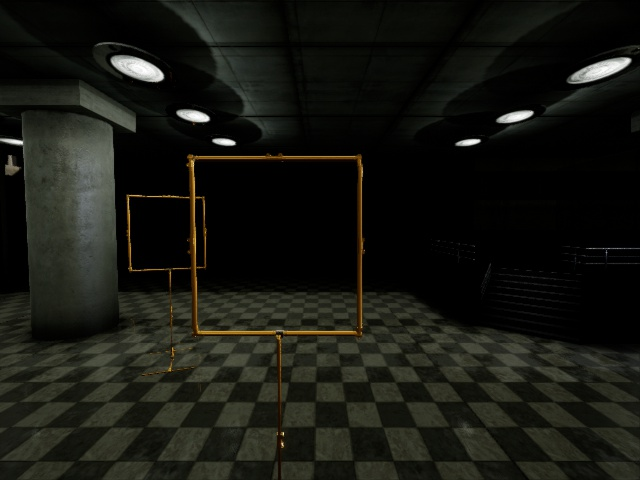
\includegraphics[width=\textwidth]{fig/gate_example}
	\end{minipage}
\begin{minipage}{0.33\textwidth}
	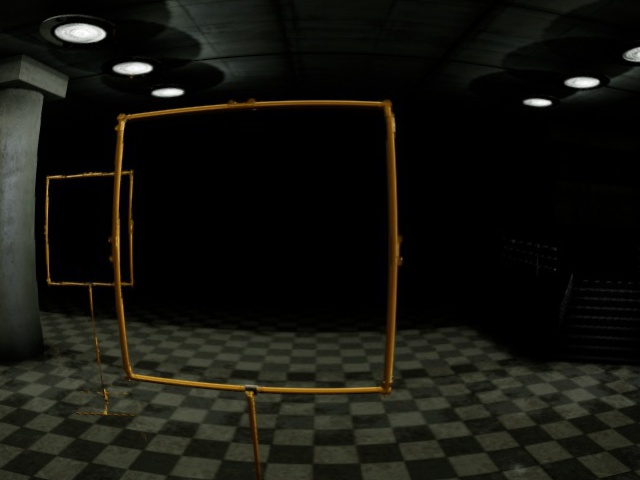
\includegraphics[width=\textwidth]{fig/gate_example_distorted}
\end{minipage}
\begin{minipage}{0.33\textwidth}
	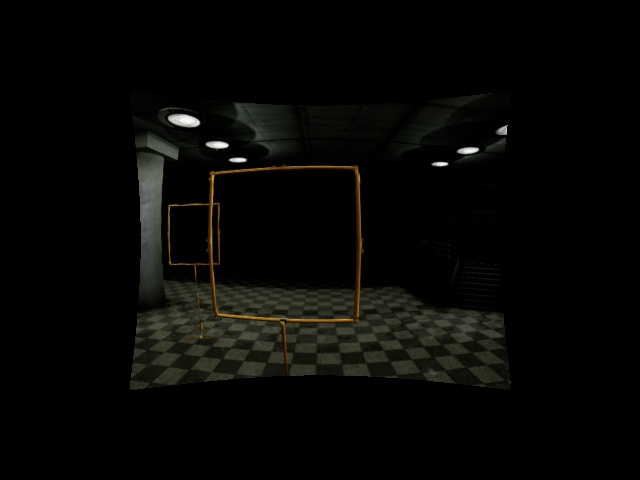
\includegraphics[width=\textwidth]{fig/gate_example_undistorted}
\end{minipage}
\caption{Example Lens Distortion. Original scene (left), distorted view (center), undistorted view (right)}
\label{fig:distortion}
\end{figure}

\paragraph{Chromatic Aberration.}

Similarly to \cite{Carlson2018}, chromatic aberration is applied by scaling the locations of the green channel, as well as applying translations on all channels. The model can be implemented as affine transformation of the pixel locations for each channel:

\begin{equation}
\begin{pmatrix}
x' \\
y' \\
1
\end{pmatrix} = \begin{pmatrix}
S & 0 & t_x \\
0 & S & t_y \\
0 & 0 & 1
\end{pmatrix} \begin{pmatrix}
x \\
y \\
1
\end{pmatrix}
\end{equation}

\begin{figure}[htbp]
	\centering
	\begin{minipage}{0.49\textwidth}
		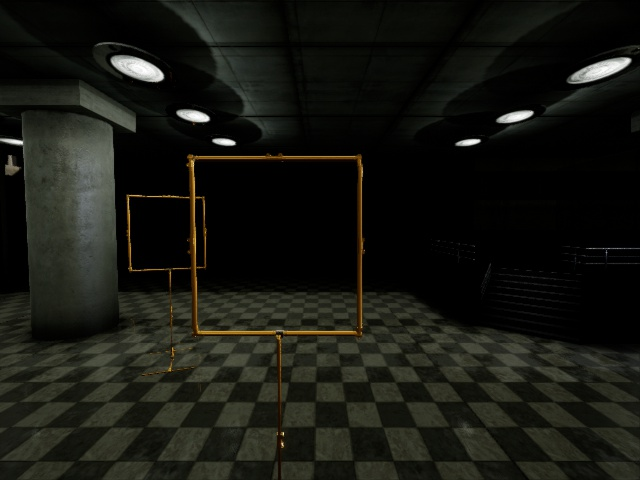
\includegraphics[width=\textwidth]{fig/gate_example}
	\end{minipage}
	\begin{minipage}{0.49\textwidth}
		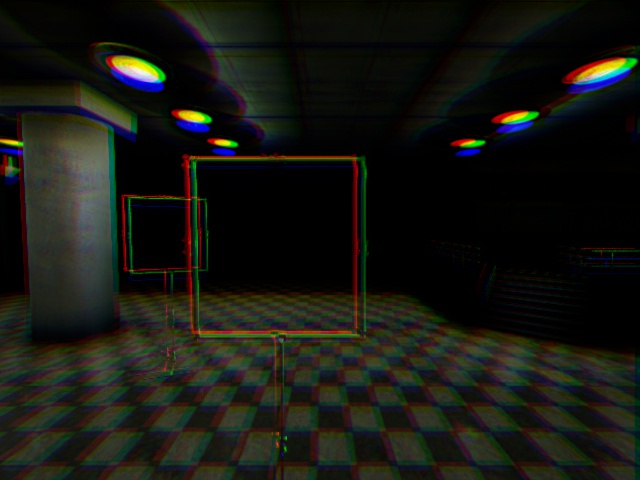
\includegraphics[width=\textwidth]{fig/gate_example_chromatic}
	\end{minipage}
	\caption{Example Chromatic Aberration with $S=[1, 1.01, -5.0]$, $t_x=[10,0.1,0.01]$, $t_y=[0.1,-0.1,0.0.01]$. Original scene (left), after transformation (right)}
	\label{fig:chromatic}
\end{figure}


\paragraph{Motion Noise.}

Motion blur is a phenomenon depending on camera properties as well as the motion of camera and objects. Although a full modelling of this process might benefit the learning process, it requires a complex pipeline and is computationally expensive. Therefore a strong simplification is used, namely a one-dimensional Gaussian median filter:

\begin{equation}
K_v = \begin{pmatrix}
...				 \\
\mathcal{N}(\mu-1) \\
\mathcal{N}(\mu)  \\
\mathcal{N}(\mu+1)	 \\
	...					
\end{pmatrix} \quad
K_h = \begin{pmatrix}
...	& \mathcal{N}(\mu-1)	&	\mathcal{N}(\mu) &	\mathcal{N}(\mu+1) & ...\\
\end{pmatrix}
	\label{eq:motion_noise}
\end{equation}

Where $\mathcal{N}$ is a Gaussian-PDF with mean $\mu$ and variance $\sigma$,  $K_v$ models vertical motion blur, $K_h$ horizontal motion blur. The size of the kernel is chosen by $k$.

\begin{figure}[htbp]
	\begin{minipage}{0.33\textwidth}
		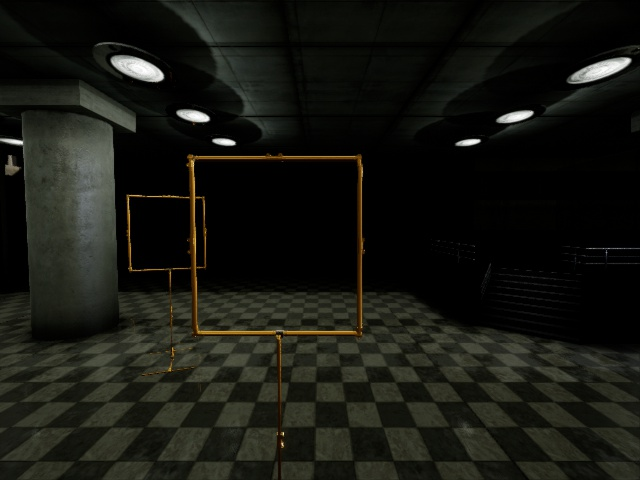
\includegraphics[width=\textwidth]{fig/gate_example}
	\end{minipage}
	\begin{minipage}{0.33\textwidth}
		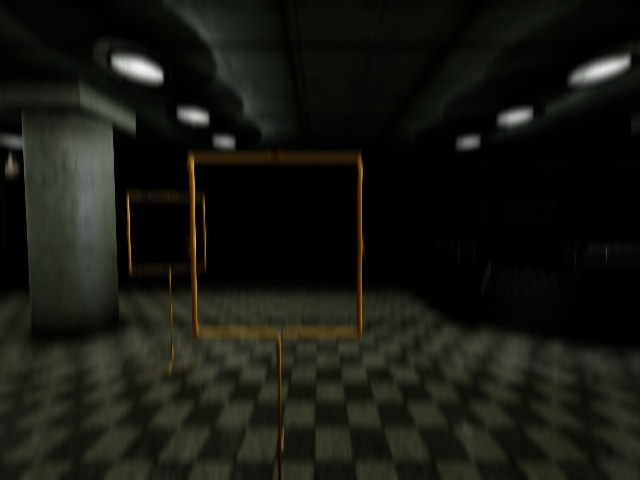
\includegraphics[width=\textwidth]{fig/gate_example_motionblur_v}
	\end{minipage}
	\begin{minipage}{0.33\textwidth}
		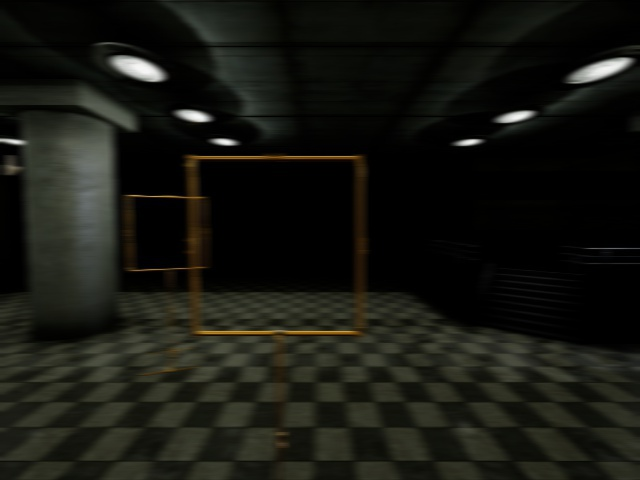
\includegraphics[width=\textwidth]{fig/gate_example_motionblur_h}
	\end{minipage}
	\caption{Example Motion Blur with $k=15$, $\sigma=5.0$. Original scene (left), vertical movement (center), horizontal movement (right)}
	\label{fig:motionblur}
\end{figure}


\paragraph{Out-of-focus Blur.}

Next to motion, sensor noise can lead to blurry images. For the blur operation a 2D Gaussian kernel is applied on the input image with:

\begin{equation}
 k = \frac{1}{2\sigma_x\sigma_y\pi}e^{-\sqrt{\frac{x^2 + y^2}{2\sigma_x\sigma_y}}} 
\end{equation}

\begin{figure}[htbp]
	\centering
	\begin{minipage}{0.49\textwidth}
		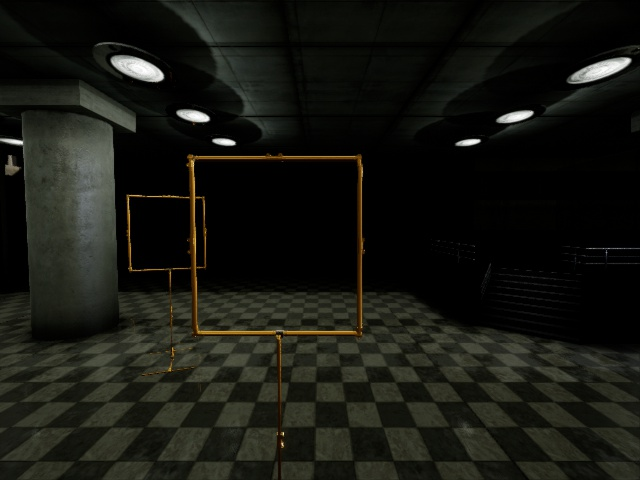
\includegraphics[width=\textwidth]{fig/gate_example}
	\end{minipage}
	\begin{minipage}{0.49\textwidth}
		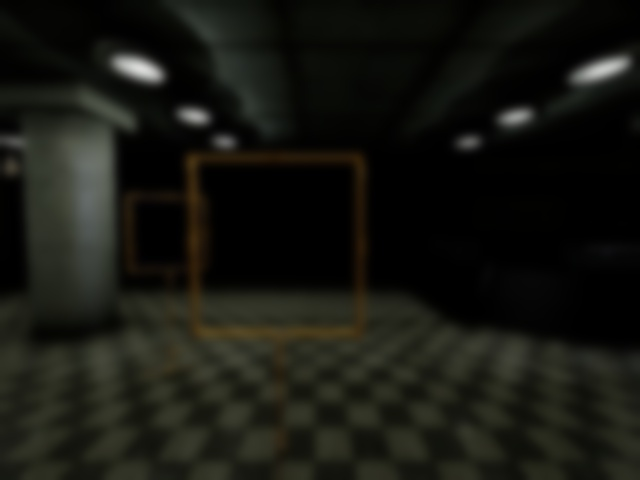
\includegraphics[width=\textwidth]{fig/gate_example_focusblur}
	\end{minipage}
	\caption{Example Out-of-Focus blur.}
	\label{fig:focusblur}
\end{figure}

\paragraph{Exposure.}

With the exposure model:
 
\begin{equation}
 I = f(S) = \frac{255}{1 + e^{-A S}}
\end{equation}
where $A$ is a constant term for contrast and $S$ the exposure.

Following the model from \cite{Carlson2018} the image is re-exposed using:

\begin{equation}
	I' = f(S+\Delta S)
\end{equation}

where $S$ is obtained from :
\begin{equation}
S = f^{-1}(I) = \frac{\ln(\frac{255}{I}-1)}{-A}
\end{equation}

\begin{figure}[htbp]
	\centering
	\begin{minipage}{0.49\textwidth}
		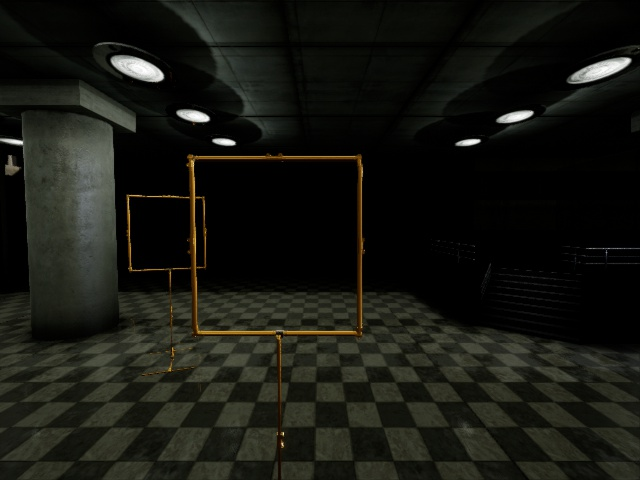
\includegraphics[width=\textwidth]{fig/gate_example}
	\end{minipage}
	\begin{minipage}{0.49\textwidth}
		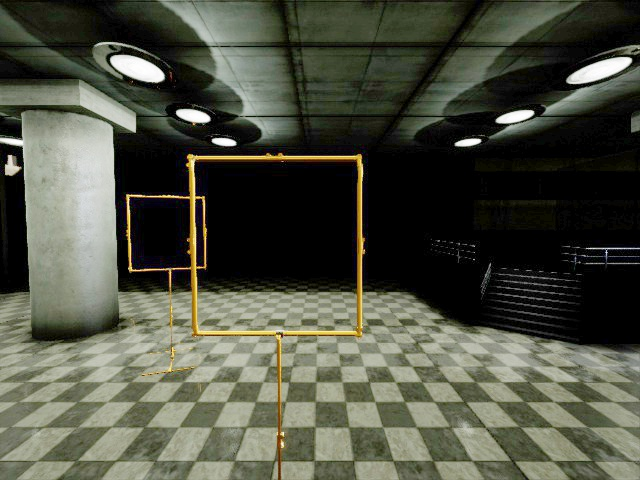
\includegraphics[width=\textwidth]{fig/gate_example_exposure}
	\end{minipage}
	\caption{Example Exposure with $\Delta S = 2.0$, $A = 1.0$.}
	\label{fig:exposure}
\end{figure}

\paragraph{Noise.}


\subsection{Artificial Augmentation}

Inspired by \cite{Howard2013, Redmon, Liu} the application of several artificial image transformations is studied. The overall goal is to generate more variations in the input signal and thus to make the model more invariant against changes in those properties. We do not use image scaling or translation for augmentation as it is easier to incorporate such variations using the motion model.

\paragraph{Brightness.} In order to obtain a model that is more robust against illumination changes image brightness is alternated. Therefore a scaling on the V-channel in HSV-colour space is applied. The scaling is drawn from a uniform distribution in between $b_1$ and $b_2$.
	
\paragraph{Grayscale.} By transforming a subset of samples into grayscale images, the model is forced to learn more color invariant features. A grayscale conversion is applied with a probability of $g$.
	
\paragraph{Histogram Equalization.} Changes in the environmental conditions can also affect contrast. By applying a histogram equalization on a subset of images, variations in contrast are achieved. \todo{histeq}
	
\paragraph{Flip.} By mirroring the image vertically, more variations in object locations are achieved. The operation is applied with a probability of $f$.


\subsection{Hypothesis}
\label{sec:training:hypothesis}

Transfer to real should be easier if complexity can be modelled

Most of described approaches in \Cref{sec:training:related} focus on objects that have complex structures and therefore provide robust features that are independent of the rest of the scene. For example a face contains eyes and a nose, which appearances are influenced to some extend by light conditions but relatively independent from image background. It has been shown in \todoref{visualizing cnns} how object detectors exploit this kind of structure in the learned representation. We hypothesize that a model to detect such complex objects is less domain dependent and can therefore be more easily transferred to domains with other environmental conditions. That is the performance drop $\Delta m$ of a model trained in $S$ and applied in $T$ where $S$ and $T$ are different in terms of environmental conditions will be larger for an \ac{EWFO} than for a more complex object.

If the environmental conditions have an high impact, their modelling is particularly important in the data generation process. We hypothesize that, as pasting the image on random backgrounds fails to capture these conditions, it is not a sufficient method to train a model for the detection of \acp{EWFO}. That is the performance drop $\Delta m$ of a model trained in $S$ and applied in $T$ where $S$ is generated by pasting a 3D-Mesh on random backgrounds and $T$ is modelled using full environment rendering will be prohibitively large.
 
From that it follows that in order to generate data for \ac{EWFO} Object Detection it is particularly important to address the domain shift. In literature two ways to approach this problem on the data level can be found: (1) providing a lot of variance in the training data to obtain a representation that is robust against domain shifts; (2) including target domain knowledge in the training data to obtain a representation that is tailored to the target domain. We hypothesize that there is a trade-off between these two approaches: A model that performs well across domains will perform poorer in a particular domain but better in other domains compared to a model that is trained for that particular domain. Hence, we hypothesize, if knowledge of $T$ is included when generating $S$ the performance in $T$ will improve given a fixed modelsize/ the model can be simplified achieving equal performance. 

In the data generation process this can be addressed on several levels:

\begin{enumerate}
	\item \textbf{Scene Generation.} A model trained for a particular room, with particular lightning conditions will perform better in that room but perform poorly in other rooms than a model trained on various rooms with various lightning conditions. By modelling the environment of the real data, the performance on the real data can be improved.
	
	\item \textbf{Camera Placement.} A model trained using the quad-rotor model will perform better on real data than a model trained using random camera locations.
	
	\item \textbf{Postprocessing.} A model trained using a post-processing pipeline that models the real-world sensor will perform better on the real data than a model that is trained on using varying parameters in the post-processing pipeline.  
\end{enumerate}

The hypotheses are summarized in the following:

\begin{enumerate}
	\item[$\mathcal{H}_1$] The performance drop $\Delta m$ of a model trained in $S$ and applied in $T$ where $S$ and $T$ are different in terms of environmental conditions will be larger for an \ac{EWFO} than for a more complex object.
	
	\item[$\mathcal{H}_2$] In contrast to a more complex object, the performance drop $\Delta m$ of a model for the detection of \acp{EWFO} trained in $S$ and applied in $T$ where $S$ is generated by pasting a 3D-Mesh on random backgrounds and $T$ is modelled using full environment rendering will be prohibitively large.
	
	\item[$\mathcal{H}_3$] A model trained in $S_0$ where $S_0 \in S$ and applied in $T_0$, where $S_0 = T_0$ will perform better in $T_0$ than a model that is trained in $S$ but perform worse in $T_1$ where $T_1 \in S$ and $T_1 \neq S_0$. 

	\item[$\mathcal{H}_3$] By including properties of $T$ in $S$ where $S$ is an artificial set $T$ is the real data, the performance $m_T$ of a model can be improved. 

\end{enumerate}

\section{Experiments}
\label{sec:training:experiments}
In order to evaluate the formulated hypotheses several experiments are conducted. The model used is the TinyYoloV3-Architecture, further described in \Cref{sec:object_detection}. The reported metrics are described in \Cref{sec:metrics}. For all experiments mean and standard deviation of 10 runs are reported.
\begin{equation}
	x = \mathcal{U}(-30,30),\quad y = \mathcal{U}(-20,20),\quad z = \mathcal{N}(-4.5,0.5)),\quad
	\phi = \mathcal{U}(0,0.1\pi),\quad \theta = \mathcal{U}(0,0.1\pi),\quad \psi = \mathcal{N}(-\pi,\pi)
	\label{eq:distroexp}
\end{equation}


\subsection{Experiment I}

In order to evaluate $\mathcal{H}_1$ a model is trained in a $S$ and applied in $T$. Three objects are investigated namely the \textit{Square-Gate}, \textit{Round-Gate} and \textit{Person.} The source environment is \textit{Basement}, the target domain is \textit{Daylight.} The training set consists of 20 000 samples, where for every batch of 2000 samples the objects are rearranged in the room. The test set consist of 1000 samples and fixed object arrangement. The view points are samples from the distributions described in the following:
$$
x = \mathcal{U}(-30,30),\quad y = \mathcal{U}(-20,20),\quad z = \mathcal{N}(-4.5,0.5)
$$
$$
\phi = \mathcal{U}(0,0.1\pi),\quad \theta = \mathcal{U}(0,0.1\pi),\quad \psi = \mathcal{N}(-\pi,\pi)
$$
Where $ \mathcal{U}(a,b)$ is a uniform distribution between $a,b$ and $\mathcal{N}(\mu,\sigma^2)$ is a Gaussian distribution with mean $\mu$ and variance $\sigma^2$.
The parameters are chosen experimentally aiming to resemble common view points of a person standing in the room.


\subsection{Experiment II}

In order to evaluate $\mathcal{H}_2$ a model is trained in a $S$ and applied in $T$. Three objects are investigated namely the \textit{Square-Gate}, \textit{Round-Gate} and \textit{Person.}  The training set consists of 20 000 samples, where for every batch of 2000 samples the objects are rearranged in the room. The test set consist of 1000 samples and fixed object arrangement. The training set is generated by replacing the background with images samples from the Pascal VOC dataset. The test set is taken in \textit{Daylight} Environment. The view points are samples from the distributions described in the following:

Where $ \mathcal{U}(a,b)$ is a uniform distribution between $a,b$ and $\mathcal{N}(\mu,\sigma^2)$ is a Gaussian distribution with mean $\mu$ and variance $\sigma^2$.
The parameters are chosen experimentally aiming to resemble common view points of a person standing in the room.

\subsection{Experiment III}

In order to evaluate $\mathcal{H}_3$ the individual domain properties and their incorporation in the data generation process are studied. Each property is compared in terms of specialization and generalization. That is the property are varied between three configurations: (1) Resembling the target domain, (2) Generalizing across domains, (3) Disabled (if applicable).

The test set is generated in the environment \textit{IROS}, using the quad-rotor model. In total 1000 images are sampled taken from one trajectory. The post-processing applies:
\begin{enumerate}
	\item Lense distortion
	\item Chromatic Abberration
	\item Motion Blur
	\item Out-of-Focus Blur
	\item Exposure
\end{enumerate}

\subsection{Experiment IV}

In order to evaluate $\mathcal{H}_4$ the individual domain properties are measured on the target domain and incorporated in the training set.


\section{Results}
\label{sec:training:results}

\section{Discussion}
\label{sec:training:discussion}

\section{Conclusion}
\label{sec:training:conclusion}


